\documentclass{standalone}
\usepackage{tikz}
\usetikzlibrary{arrows.meta, positioning}

\begin{document}

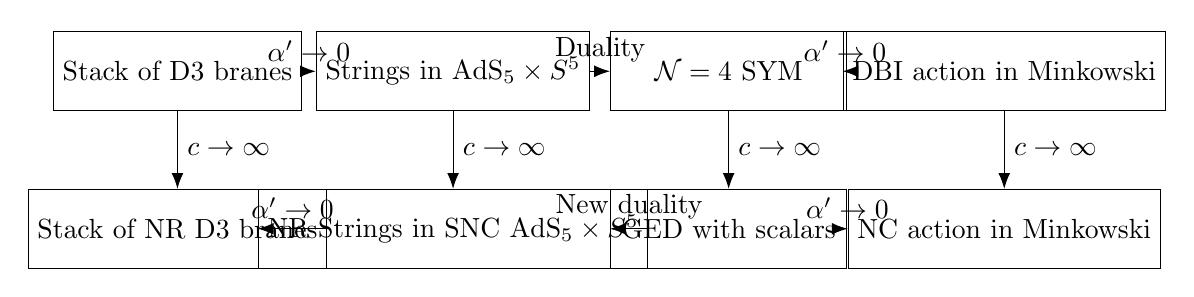
\begin{tikzpicture}[node distance=2.5cm, auto]
    % Styles
    \tikzstyle{block} = [rectangle, draw, minimum width=3cm, minimum height=1cm]
    \tikzstyle{line} = [draw, -{Latex[length=2mm]}]

    % Nodes
    \node [block] (stackD3) {Stack of D3 branes};
    \node [block, right of=stackD3, node distance=3.5cm] (stringsAdS) {Strings in AdS$_5 \times S^5$};
    \node [block, right of=stringsAdS, node distance=3.5cm] (n4SYM) {$\mathcal{N} = 4$ SYM};
    \node [block, right of=n4SYM, node distance=3.5cm] (dbiAction) {DBI action in Minkowski};

    \node [block, below of=stackD3, node distance=2cm] (stackNRD3) {Stack of NR D3 branes};
    \node [block, right of=stackNRD3, node distance=3.5cm] (nrStringsSNC) {NR Strings in SNC AdS$_5 \times S^5$};
    \node [block, right of=nrStringsSNC, node distance=3.5cm] (gedScalars) {GED with scalars};
    \node [block, right of=gedScalars, node distance=3.5cm] (ncMinkowski) {NC action in Minkowski};

    % Arrows
    \path [line] (stackD3) -- node [above] {$\alpha' \to 0$} (stringsAdS);
    \path [line] (stringsAdS) -- node [above] {Duality} (n4SYM);
    \path [line] (n4SYM) -- node [above] {$\alpha' \to 0$} (dbiAction);

    \path [line] (stackNRD3) -- node [above] {$\alpha' \to 0$} (nrStringsSNC);
    \path [line] (nrStringsSNC) -- node [above] {New duality} (gedScalars);
    \path [line] (gedScalars) -- node [above] {$\alpha' \to 0$} (ncMinkowski);

    % Vertical lines
    \path [line] (stackD3) -- node [right] {$c \to \infty$} (stackNRD3);
    \path [line] (stringsAdS) -- node [right] {$c \to \infty$} (nrStringsSNC);
    \path [line] (n4SYM) -- node [right] {$c \to \infty$} (gedScalars);
    \path [line] (dbiAction) -- node [right] {$c \to \infty$} (ncMinkowski);
\end{tikzpicture}

\end{document}